\chapter{Pointer and Effect Analysis}
\label{chap:pointer}
The problem of analyzing pointers is closely related to the field of effects
analysis. Indeed, establishing the relations between pointers require
understanding how and to what values fields are written to. Because of this
strong inter-dependence, it is often profitable to perform both simultaneously.

Our analysis builds summaries of methods, both in terms of effects and shape of
the heap. Those summaries are stored in graphs. In order that compute the
resulting graphs for each method, we perform a flow-sensitive
abstract-interpretation based analysis. A graph is thus associated to each
program point. The next section describes how those graphs are generated and
what their semantics are. This representation is similar in many aspects to
the graph representation used by Alexandru Salcianu in his Thesis. We can %FIXME
however point out two important differences: his work is primarily focused on
escape analysis, our isn't and thus we do not keep escape-specific information
in our abstract representation. We also introduced multiple kinds of global
nodes, that were not present in his work since it would be redundant for escape
analysis. Although the representations are similar, the semantics of our graphs
as well as the procedures to build them differ.

\begin{lstlisting}
\end{lstlisting}


\section{Graph Semantics}
Our representation is based on labelled directed graphs augmented with some
metadata. They are defined by:
\begin{eqnarray*}
    G           := &\langle& N \subseteq Nodes, \\
                   && E \subseteq Edges, \\
                   && locVar \subseteq Variables \times \mathcal{P}(N), \\
                   && Ret \subseteq N ~ \rangle \\
    Edges       := && IEdges \cup OEdges  \\
    IEdges      := && \langle N, f, N \rangle \in Nodes \times Fields \times Nodes ~\textsf{ Inside Edges } \\
    OEdges      := && \langle N, f, N \rangle \in Nodes \times Fields \times Nodes ~\textsf{ Outside Edges } \\
    Variables   := && \textsf{All local variables and arguments} \\
    Fields      := && \textsf{Field names} \\
    Nodes       := && \{ GBNode, NNode \} \cup INodes \cup LNodes \\
                   && \cup PNodes \cup OBNodes \cup LitNodes \\
    INodes      := && \langle T \rangle \in TypeInfo \times ProgramPoints ~ \textsf{(Allocation node)} \\
    LNodes      := && \langle from, via, T \rangle \in Nodes \times Fields \times TypeInfo ~ \textsf{(Load node)} \\
    PNodes      := && \langle i, T \rangle  \in \mathbb{R} \times TypeInfo ~ \textsf{(Param node)} \\
    OBNodes     := && \langle T \rangle \in TypeInfo ~ \textsf{(Object Node)} \\
    LitNodes    := && \langle T \rangle \in TypeInfo ~ \textsf{(Literal values of primitive types)} \\
    NNode       := && ~ \textsf{(Null node)} \\
    GBNode      := && ~ \textsf{(Global node)} \\
\end{eqnarray*}

Nodes generally represent sets of objects (including literals of primitive
types), while edges represent may/must-point-to relations. $G$ also contains
$locVar$ which is a mapping from local variables to sets of nodes and $Ret$
consists of the set of nodes that are returned form the procedure.

We will present the abstract representations in a graphical manner. Instead of
attaching the metadata on the side, we will draw it directly on the graph using
the following convention: we draw local variables as shapeless nodes, with an
each to each node they point to, drawn in blue. Return nodes will be drawn
using double circle around nodes. Inside edges will be drawn using a full edge,
while outside edges will be dashed. To illustrate this, we represent in
Figure~\ref{fig:pt:graph1} a simplified graph corresponding to
\begin{eqnarray*}
    G &=& \langle \{n1, n2, n3 \}, \{ e1, e2, e3 \}, [ obj \mapsto \{n1\}, this \mapsto \{n2\}, tmp \mapsto \{ n1, n3 \} ], \{n3\} \rangle  \\
    n1 &:=& INode(T),~  n2 := PNode(0, T),~ n3 := LNode(n2, f2, T) \\
    e1 &:=& IEdge(n2, f1, n1),~ e2 := IEdge(n2, f2, n3) \\
    e3 &:=& OEdge(n2, f2, n3) \\
\end{eqnarray*}

\begin{figure}[h]
    \centering

    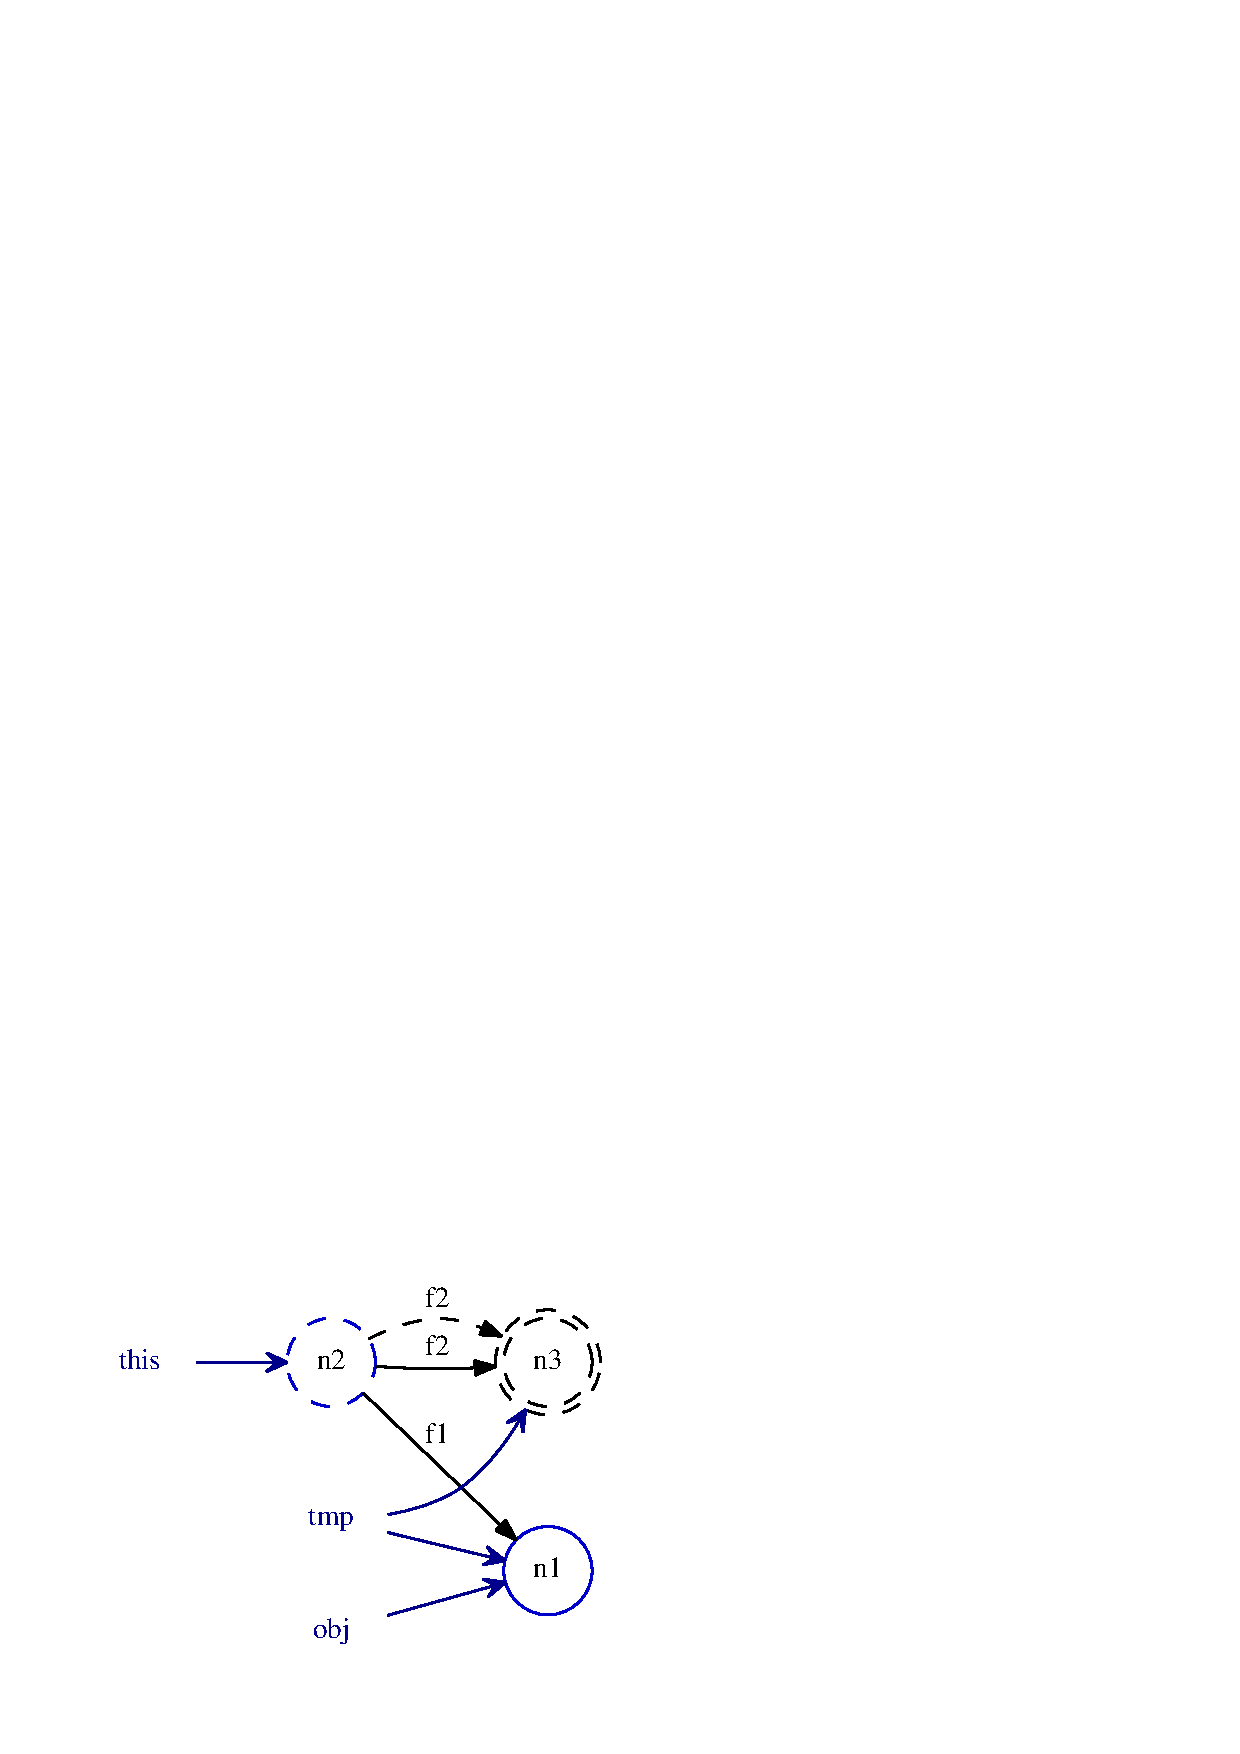
\includegraphics{images/pt_graph1}

    \caption{Simplified Graph Representation}
    \label{fig:pt:graph1}
\end{figure}

\subsection{Nodes}
As stated earlier, nodes represent sets of objects. Independently of their
kind, each node carry two pieces of information:
\begin{itemize}
    \item The type information $TypeInfo$, corresponding to the runtime types
    of the objects represented by the nodes.
    \item A \emph{singleton} flag, indicating whether the node represents only
    one object or may represent more than one. For instance, an allocation in a
    loop will yield multiple objects at the same allocation site.
\end{itemize}
We now quickly describe each kind of node and what their general meaning in a
graph is. Each kind of node will be accompanied with the actual graphical
representation, so that nodes are easily recognizable from the following
examples.

\paragraph{Inside Nodes}
Inside nodes (INodes) represent objects explicitely allocated via a \verb=new T=
statement. The graph will thus contain one \emph{INode} per allocation site.
The type of this node is exactly the allocated type (\verb=T=).
\begin{figure}[h]
    \centering

    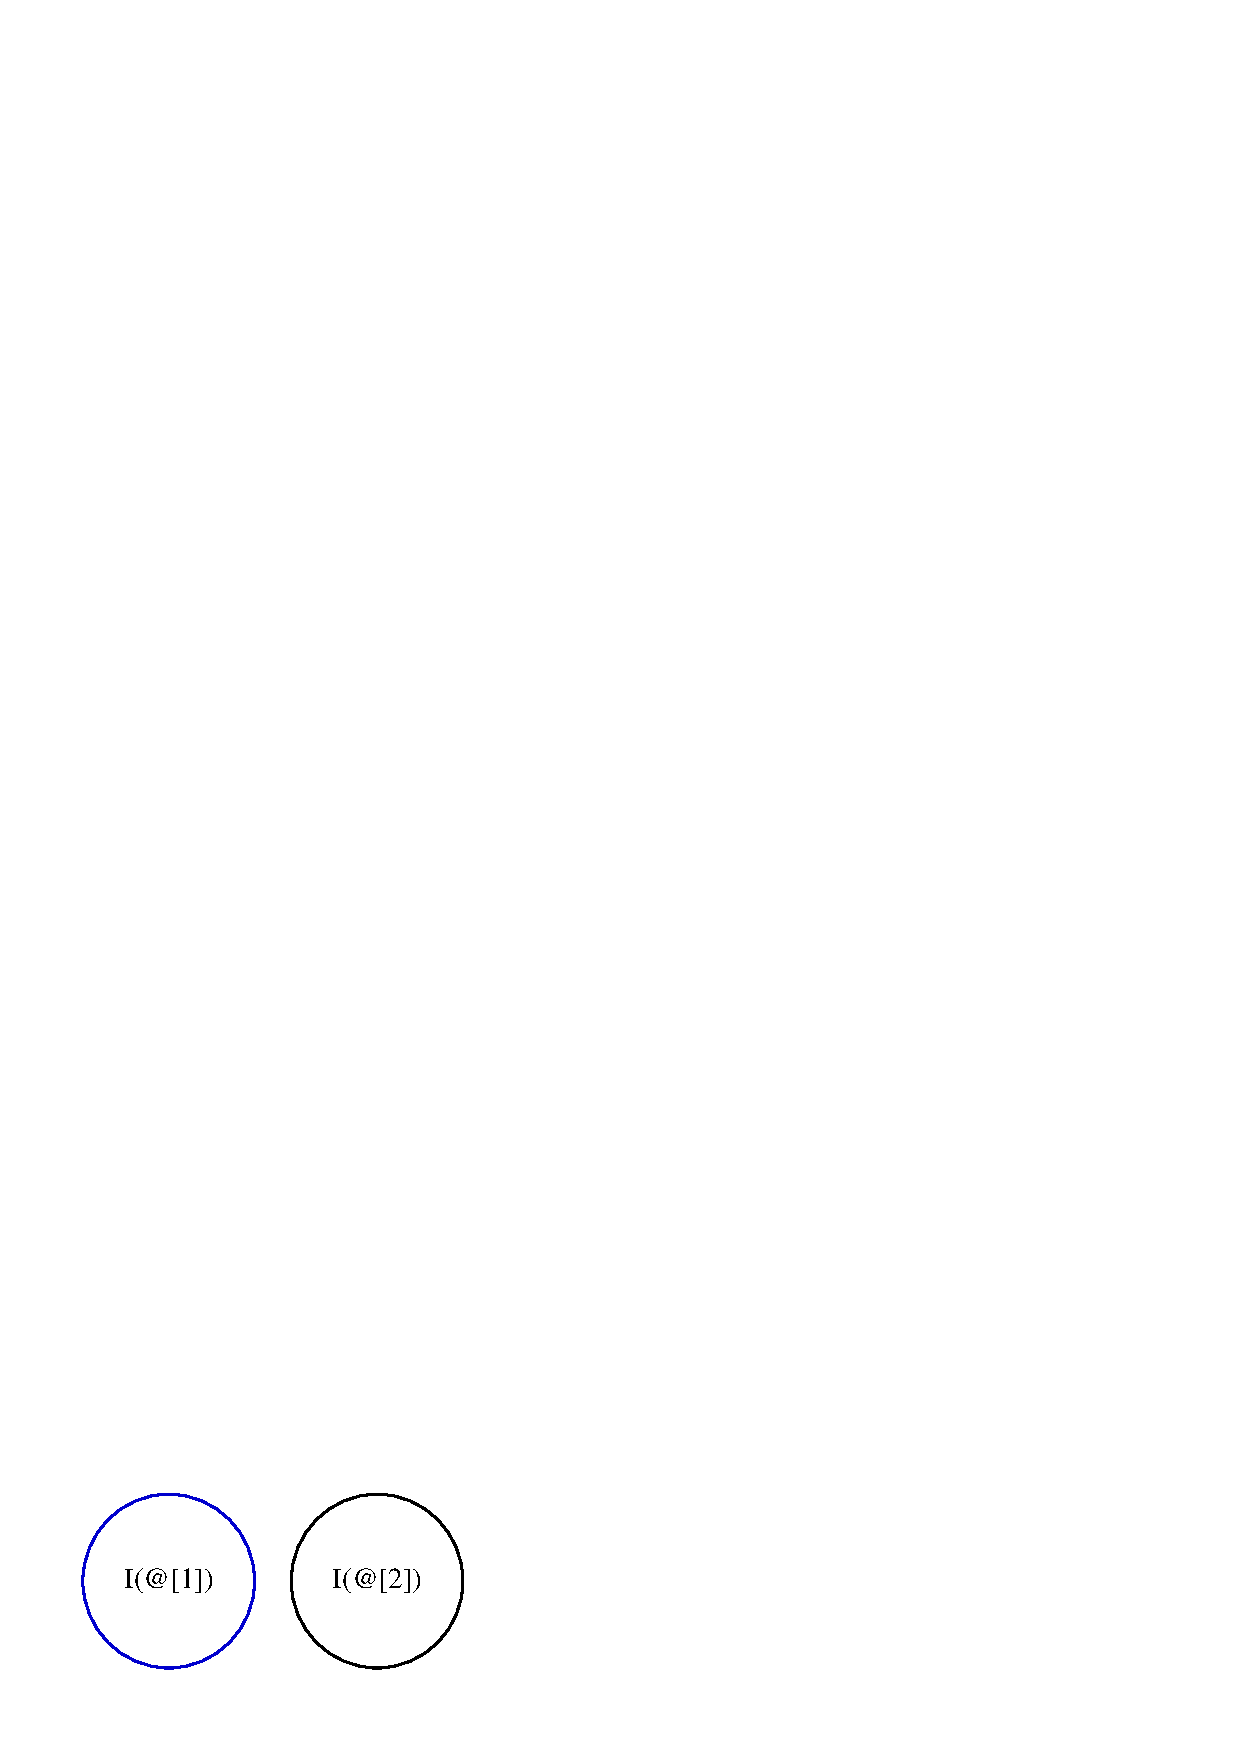
\includegraphics{images/pt_inodes}

    \caption{Two inside nodes at program points $@1$ and $@2$. Blue nodes are
    singleton objects.}
    \label{fig:pt:inodes}
\end{figure}

\paragraph{Load Nodes}
Intuitively, load nodes (LNodes) represent objects that are not yet determined.
For instance, the code:
\begin{lstlisting}
    def foo(arg: A) {
        val a = arg.f
        a
    }
\end{lstlisting}
will generate a load node representing the objects that \verb/arg.f/ points to
at the time of the call to \verb/foo()/. Section~\ref{sec:pt:inlining} will
describe in full detail how we resolve load nodes when inlining the graph of
the callee into the caller. We will not introduce load nodes if we don't have
to, for instance, in the following code:
\begin{lstlisting}
    def foo(arg: A) {
        arg.f = arg
        val a = arg.f
        a
    }
\end{lstlisting}
we know that \verb/arg.f/ points to \verb/arg/, and thus we don't need to
introduce a load node. Load nodes are conservatively assuming that they may
represent many objects, and their attached type is the compile type of of the
field and all its subtypes.

\begin{figure}[h]
    \centering

    
\includegraphics{images/pt_lnodes}

    \caption{Load Nodes are always dashed. Numbers used in the representation
    are used to uniquely identify them. Load nodes are never singletons.}
    \label{fig:pt:lnodes}
\end{figure}

\paragraph{Parameter Nodes} Parameter nodes (PNodes) represent arguments of the current
procedure. Parameter nodes are indexed by the position of the argument. The object
corresponding to the current instance ($this$) is implicitely defined as the
\emph{PNode} of index 0. For example, the following function definition:
\begin{lstlisting}
class A {
    def foo(arg1: B, arg2: C) // ...
}
\end{lstlisting}
will yield three (singleton) parameter nodes: $PNode(0)$ of type A and
subtypes, $PNode(1)$ of type B and subtypes and $PNode(2)$ of type C and
subtypes.

\begin{figure}[h]
    \centering

    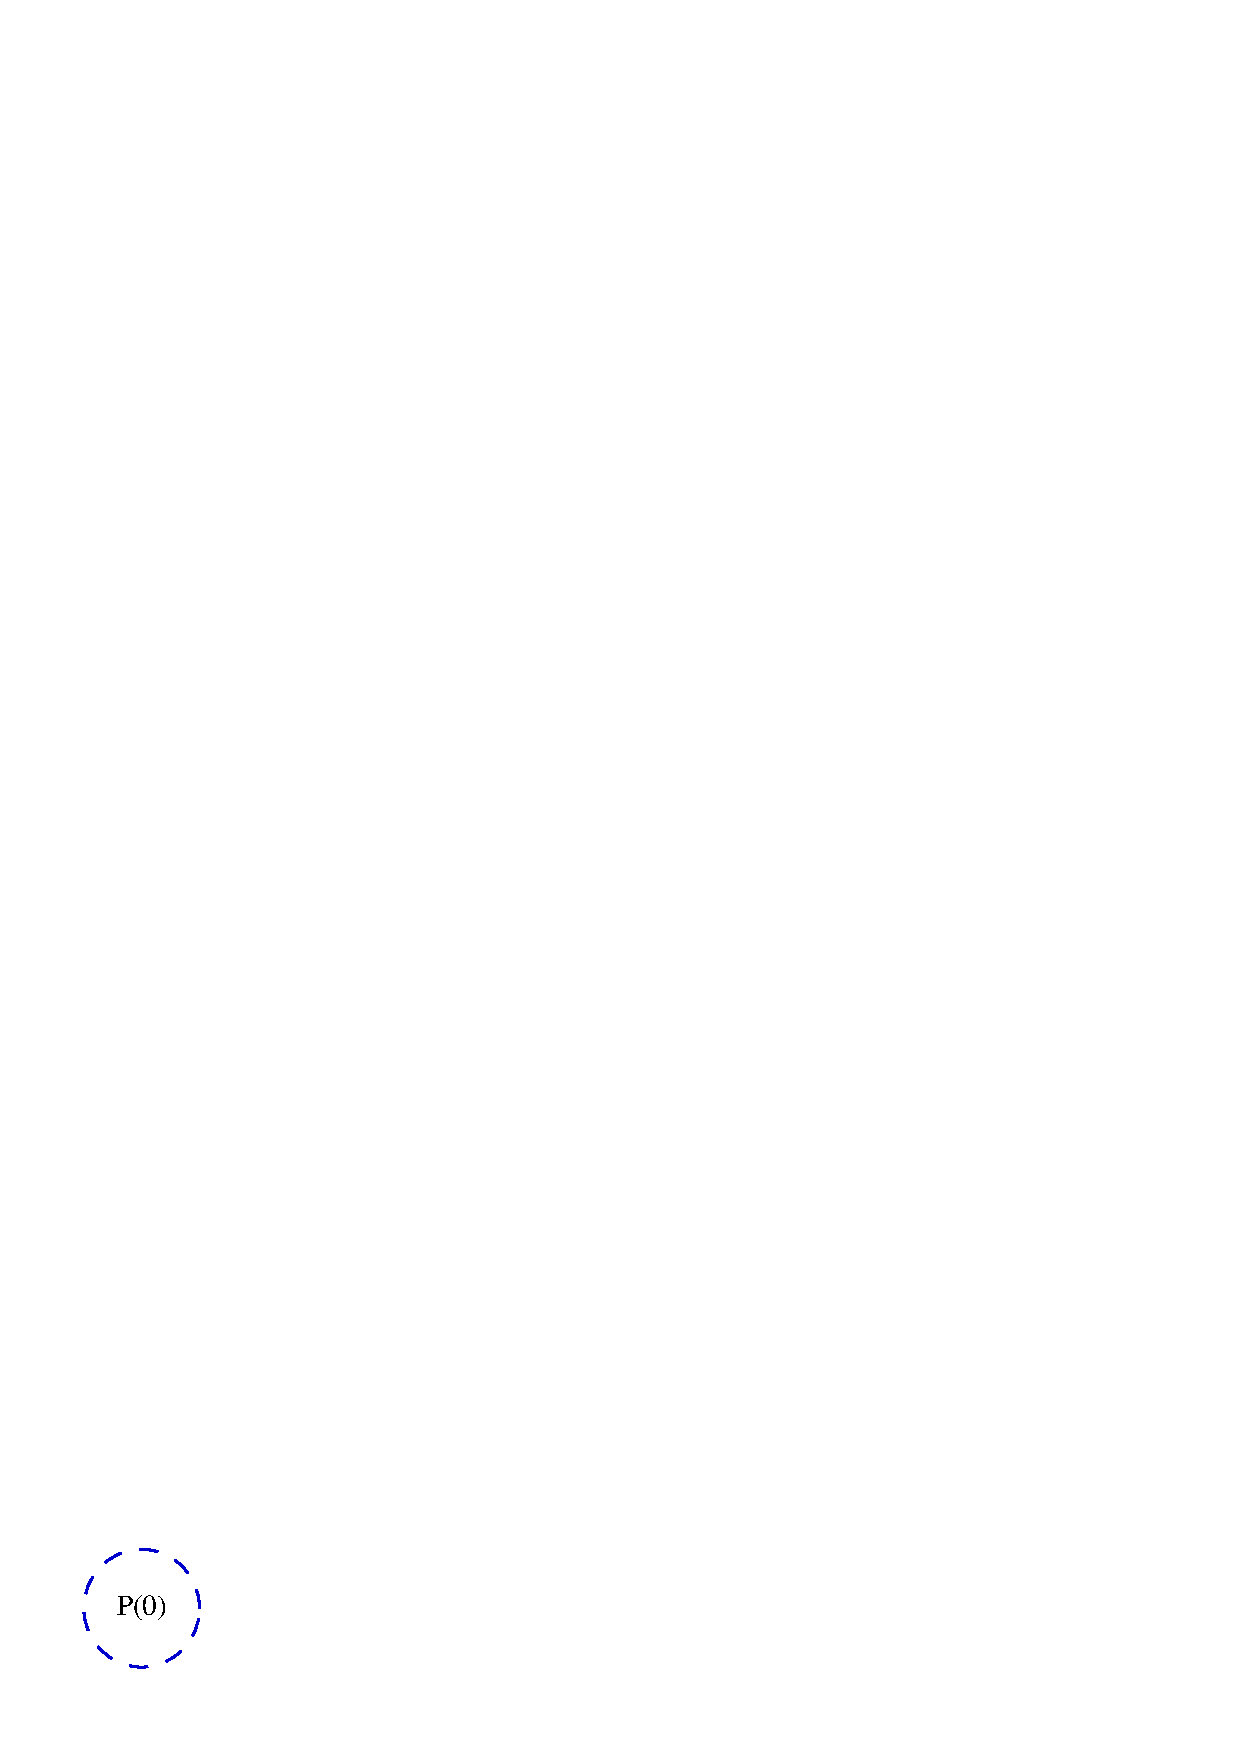
\includegraphics{images/pt_pnodes}

    \caption{Representation of a parameter node. They are always dashed and
    considered as singletons.}
    \label{fig:pt:pnodes}
\end{figure}

\paragraph{Object Nodes} Scala provides an elegant way of defining singletons
using the $object$ keyword. Object nodes (OBNodes) represent each of those
global singleton objects. Naturally, they represent a single object, and their
type information is exactly the type of the singleton.

\begin{figure}[h]
    \centering

    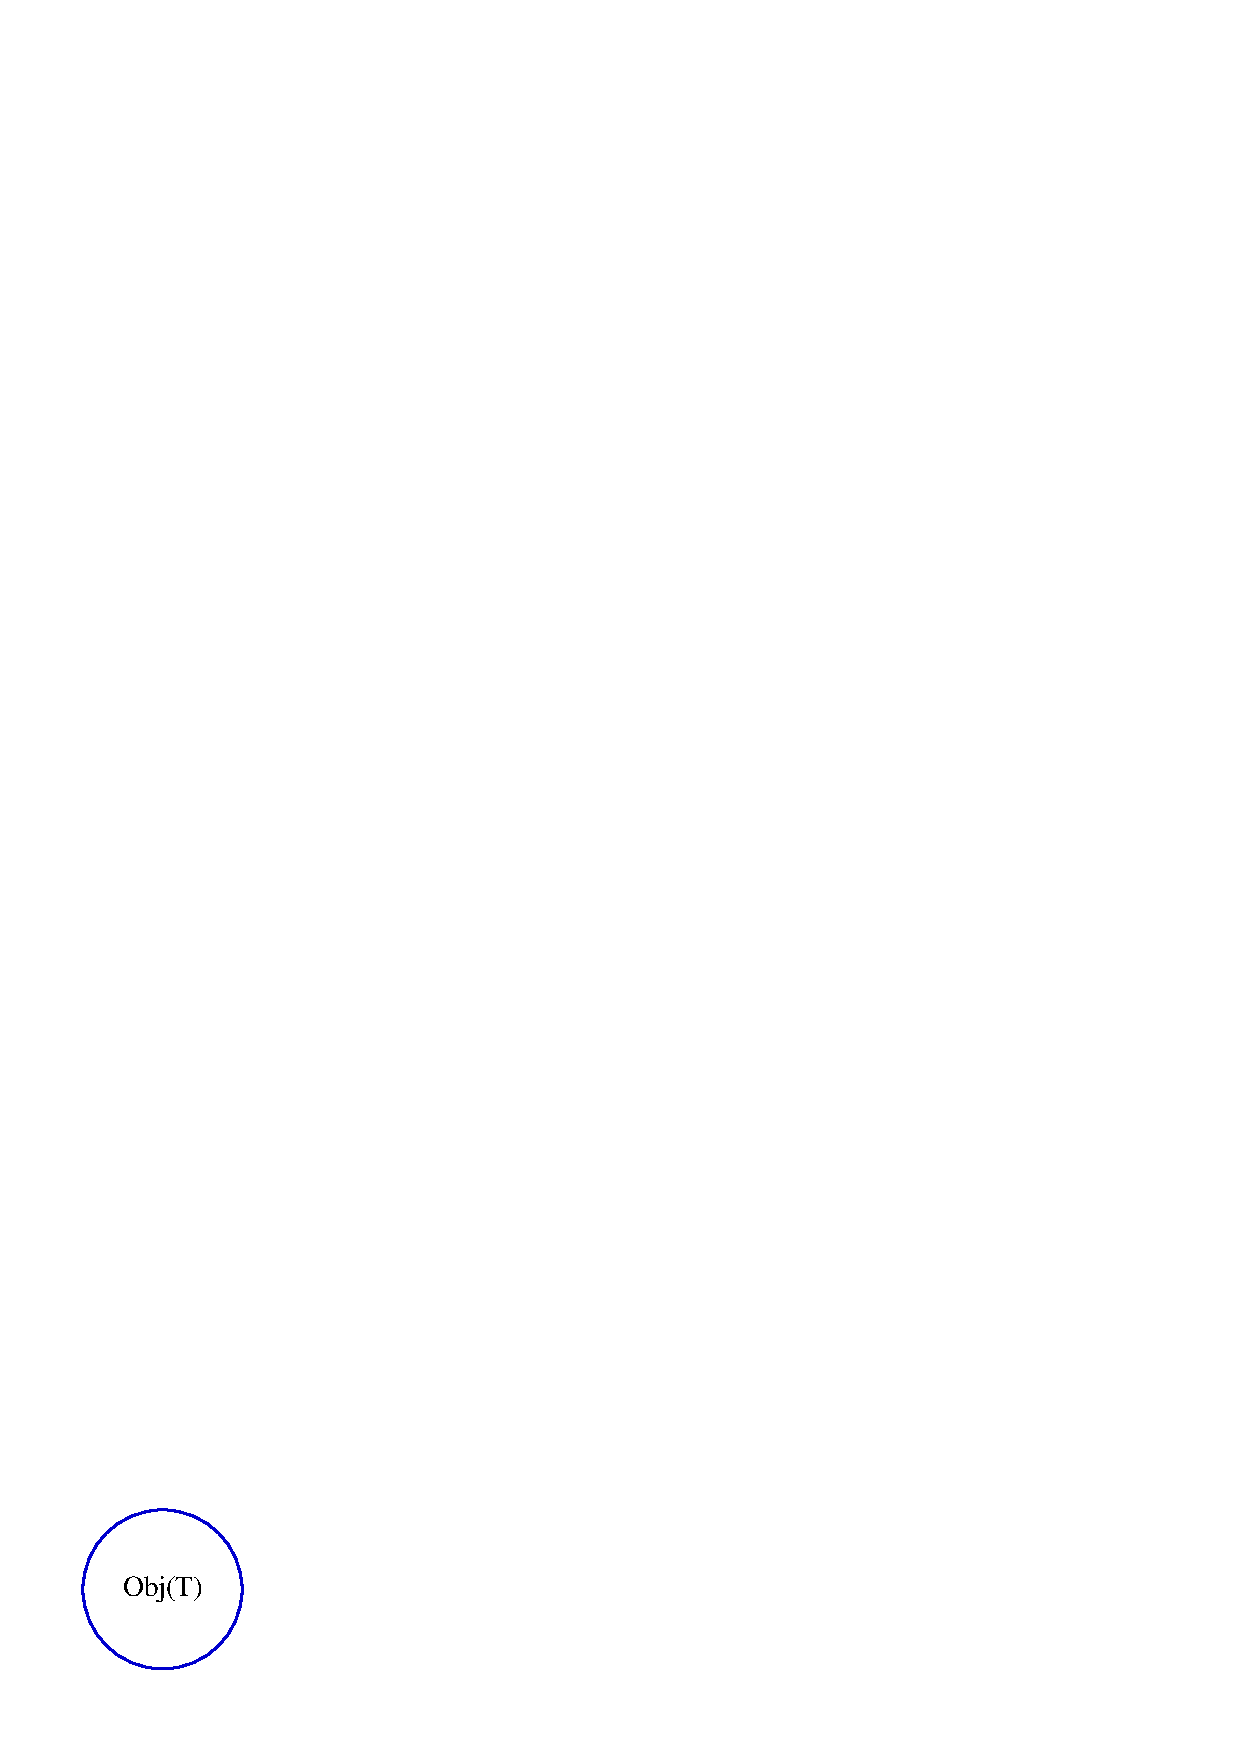
\includegraphics{images/pt_obnodes}

    \caption{Representation of a object node, always singleton.}
    \label{fig:pt:obnodes}
\end{figure}

\paragraph{Global Node} The global node (GBNode) represents all possible nodes,
it is thus of type \emph{Object} and subtypes, and is not singleton. This node
is seldomly used in error cases, and is similar to some \emph{havoc} operation.

\begin{figure}[h]
    \centering

    
\includegraphics{images/pt_gbnodes}

    \caption{Representation of a global node, of all types and never singleton.}
    \label{fig:pt:gbnodes}
\end{figure}

\paragraph{Literal Nodes} Literal Nodes represent the literal values used
within the code. Except for Strings, those values are not in fact objects.
They will thus not have any outoing edge, and are here solely to record effects
of non-object fields. Intuitively, literal node shold the type of the literal,
and are singletons. Even though they are considered as singletons, we group
every literals of the same type into the same node. The singleton flag has no
effect as there is no outgoing edges.

\begin{figure}[h]
    \centering

    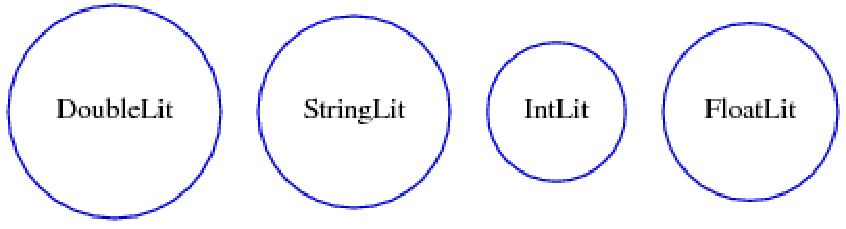
\includegraphics{images/pt_litnodes}

    \caption{Representation of some literal nodes, all singletons.}
    \label{fig:pt:litnodes}
\end{figure}


\paragraph{Null Node} The null node (NNode) represents the empty set of objects
corresponding to the $null$ value. It holds no type, and is considered singleton.

\begin{figure}[h]
    \centering

    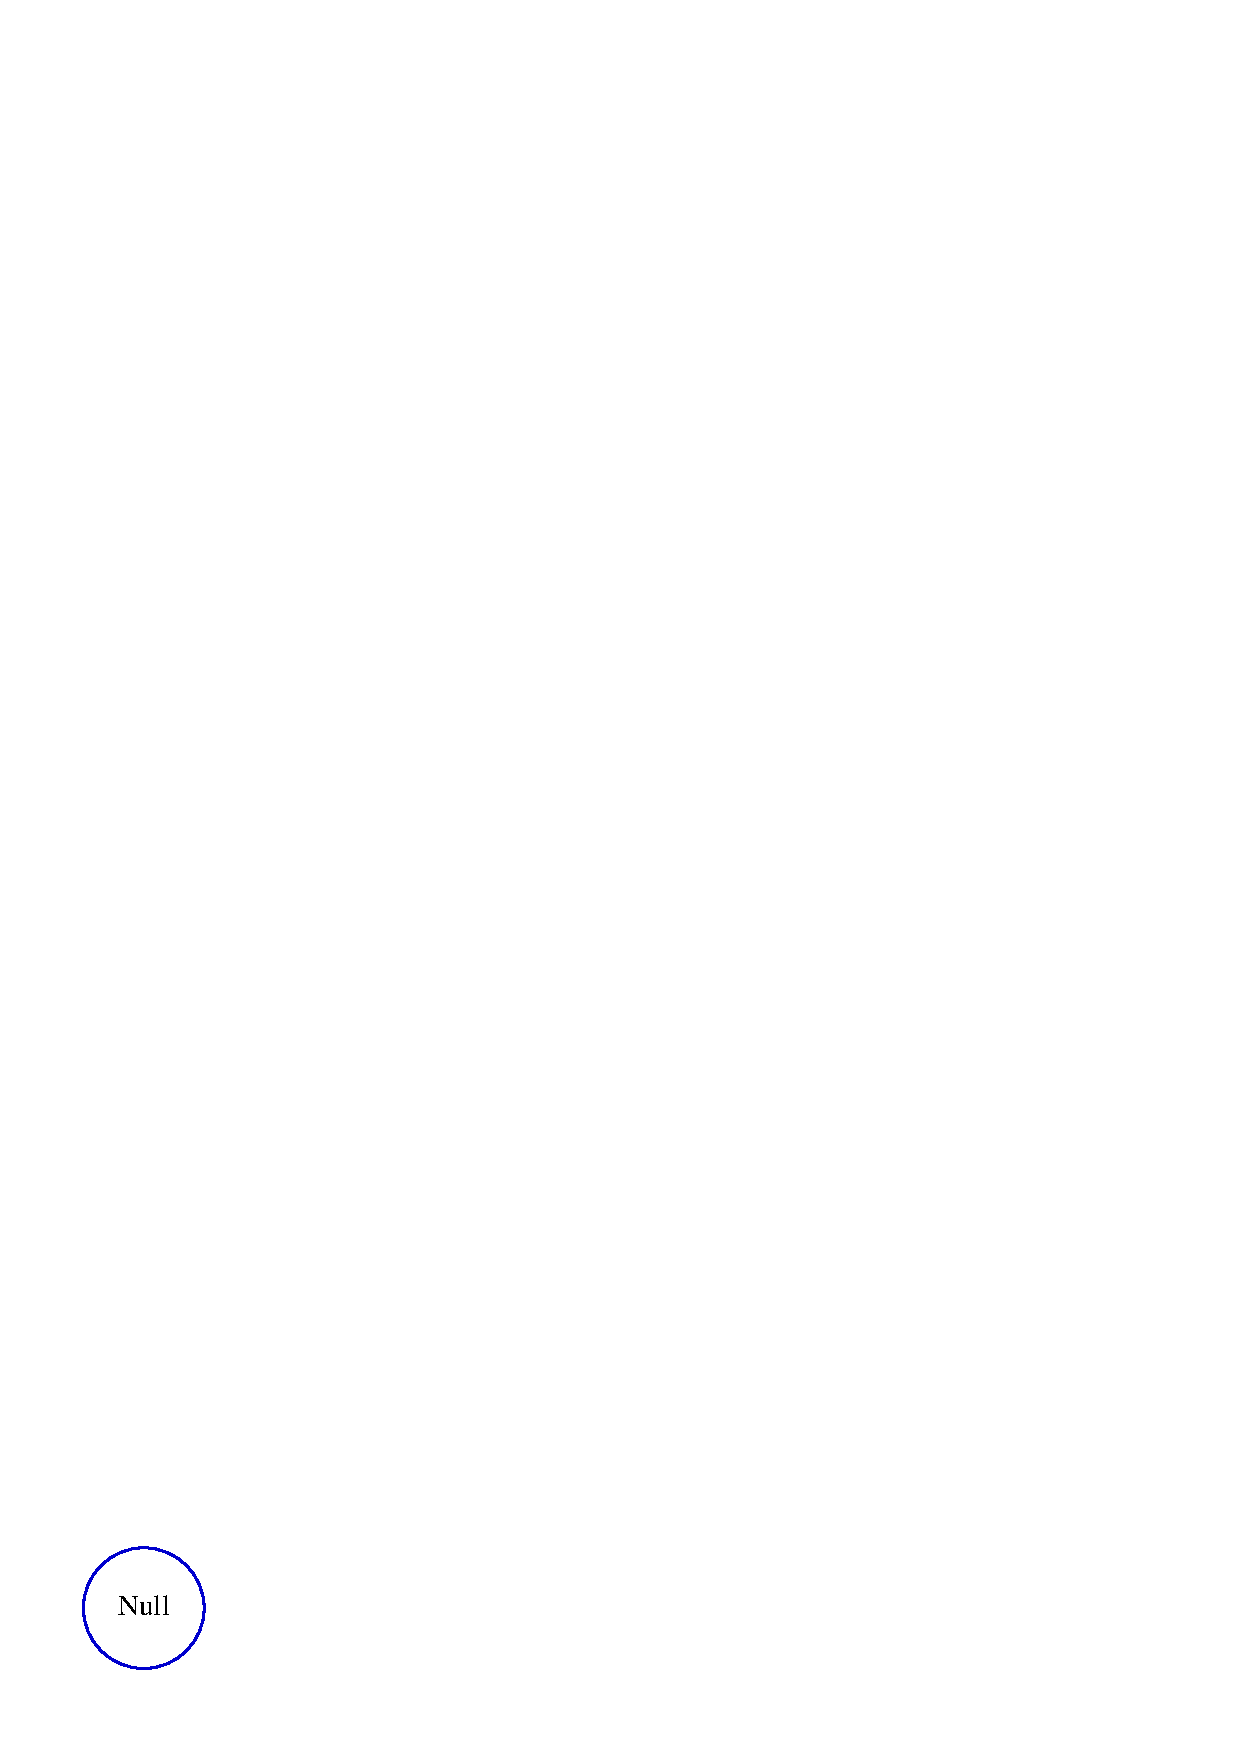
\includegraphics{images/pt_nnodes}

    \caption{Representation of a null node.}
    \label{fig:pt:nnodes}
\end{figure}

\subsection{Edges}
We distinguish two kinds of edges, \emph{inside} and \emph{outside} edges. We now
briefly describe what the meaning of each kind of edge is:

\paragraph{Inside Edges} Simply put, inside edges represent write operations to
fields. Inside edges are represented by a full arrow, labelled by the field on
which the write occurs. More than one inside edge with the same field can
originate from the same node.

\paragraph{Outside Edges} The intuition behind outside edges is that they
encode a way to reach load nodes. In other words, they represent a read on a
yet undetermined node. Outside edges are thus closely related to load nodes. In
fact, we have that every load node is reachable from a non-load node by
following outside edges only. Outside edges appear as dashed edges, labelled by
the field traversed.

To illustrate both kinds of edges, we consider in Figure~\ref{fig:pt:weak1graph} an
example of conditional update, along with the relevant parts of the resulting graph.
\begin{figure}[h]
\begin{minipage}[tl]{0.6\linewidth}
    \centering
\lstset{linewidth=0.6\linewidth}
\begin{lstlisting}
class Plop(var next: Plop) {
  def test(a: Plop) = {
    if (a != null) {
      a.next = a
    }
  }
}
\end{lstlisting}
\end{minipage}
\begin{minipage}[tr]{0.5\linewidth}
    \centering
    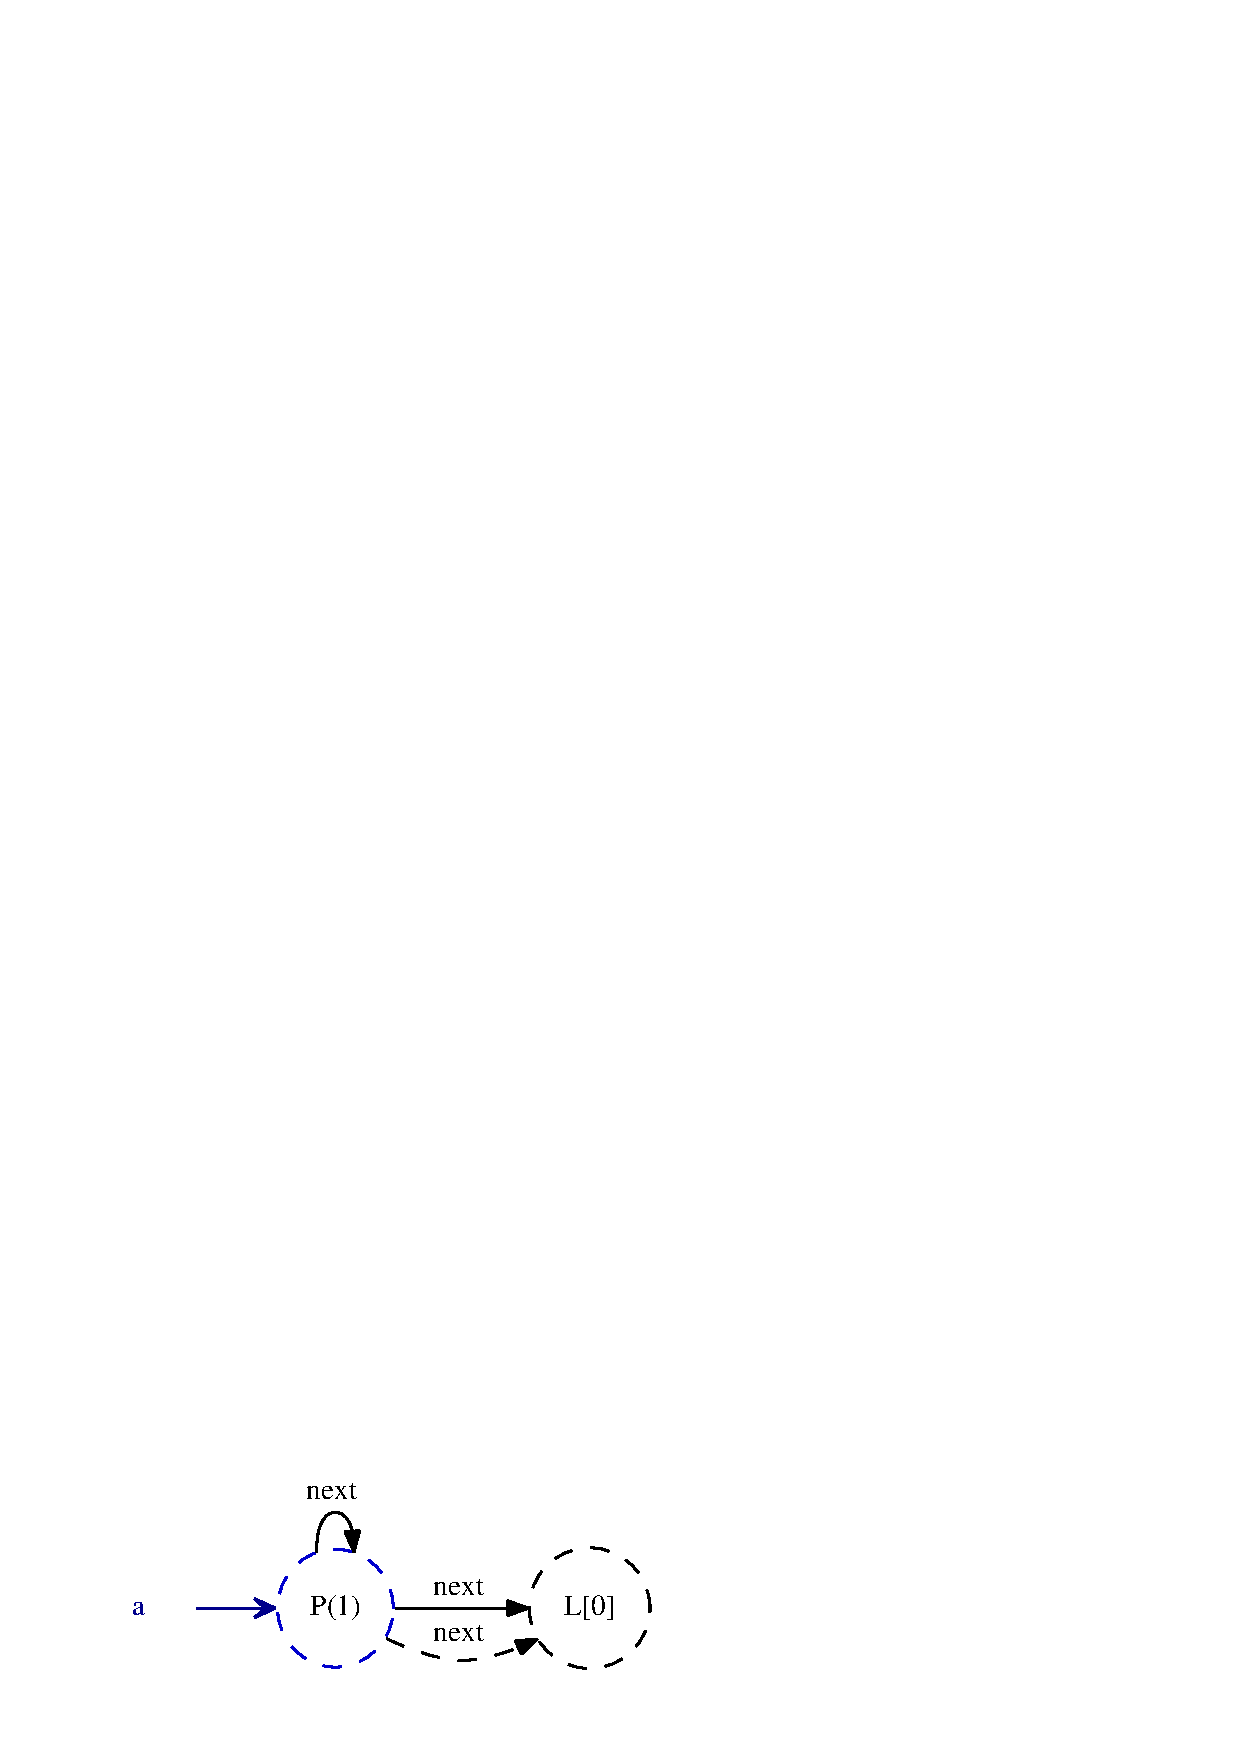
\includegraphics[scale=0.8]{images/pt_weak1graph}
\end{minipage}
    \caption{Example of weak update in code and corresponding graph}
    \label{fig:pt:weak1graph}
\end{figure}
After the call to this method, \verb/a.next/ either points to \verb/a/ or to
the old value, represented by the load node, which depends on the actual object
passed to \verb/test()/.

\FloatBarrier

Now that graphs are better defined, we provide the definitions of some utility
functions along with notations that will be used thorough this report:

\begin{eqnarray*}
    nodes(G)(v \in Variable)  &:=& G.locVar(v) \\
    types(node \in Nodes)     &:=& node.types ~\textsf{(Type information attached to the node)} \\
    singleton(node \in Nodes) &:=& node.isSingleton ~\textsf{(Whether the node represents one object)} \\
    types(G)(v \in Variable)  &:=& \bigcup \{ types(node) | node \in nodes(G)(v) \} \\
    e.v1  &:=& ~\textsf{ The source node of the edge e} \\
    e.f  &:=& ~\textsf{ The field labelling the edge e} \\
    e.v2  &:=& ~\textsf{ The destination node of the edge e} \\
\end{eqnarray*}
We will usually omit specifying the graph $G$ if it is trivially inferred from
the current context.


\section{Weak and Strong Updates}
The concept of weak or strong updates relates to the possibility for an update to
discard old values. For example, after the execution of the following code:
\begin{lstlisting}
def test() = {
    val a = new Counter
    a.value = 2
    a.value = 3
}
\end{lstlisting}
the expected value of \verb/a.value/ is 3, and never 2. In this case, the
updates are \emph{strong}: they discard previously assigned values. However, in
the following code:
\begin{lstlisting}
def test() = {
    val a1 = new A
    val a2 = new A
    val a = if (..) a1 else a2
    a.value = 2
}
\end{lstlisting}
we know that \verb/a/ points to either \verb/a1/ or \verb/a2/. It would however
be wrong to assume that \verb/a1.value/ or \verb/a2.value/ is now exclusively
2. Generally speaking, we allow a strong update for $r.f = v$ whenever $r$
represents a single object. In more formal terms, we have that the condition
for a strong update on $r.f = v$ is:
$$
    (|nodes(r)| = 1) \land ( \forall n \in nodes(r).~singleton(n) )
$$

We also have to consider strong updates performed in a branch. Consider the
following code:

\begin{lstlisting}
def test() = {
    val a = new A
    a.f = 1
    if (..) {
        a.f = 2
        a.f = 3
    }
}
\end{lstlisting}

Even though some updates are conditional, we should be able to infer that
after the branch, the value of \verb/a.f/ is either 1 or 3, but never 2. We
will describe how branches are handled with respect to strong/weak updates in
Section~\ref{sec:pt:lattice}, describing the lattice and its join operation.

In case of a weak update, we can no longer discard the old value, and we will
still need to have an inside edge pointing to it. In case it is not yet
determined by the code, we introduce as usual a load node to represent this
previous value. This load node will then be mapped to the old value, as
described in Section~\ref{sec:pt:inlining}. Figure~\ref{fig:pt:weak1graph}
represents such a case.

In order to perform a precise alias analysis, it is key to be able to perform
strong updates as often as the code allows. It is evident that discarding old
values improves the overall precision of the analysis. For instance, without
any strong update, every object field would potentially still point to null,
which is the default value of every object field directly after the allocation
of the object.

\section{Lattice Definition}
\label{sec:pt:lattice}
The lattice that we use in our effect analysis contains the graphs described
previously as elements. This time, the lattice is not point-wise as the graph
information already encompass information about every variables.

\subsection{Join Operation}
We now describe the least upper bound ($\sqcup$) operation, also commonly
referred to as \emph{join}. We generalize it to take an arbitrary number of
arguments $args := \{ a_1, ... a_n \}$. Intuitively, it is the union of all
graphs, with one exception regarding inside edges: if one node present in all
branches has an inside edge of a field originating from it in only some of the
branches, we will have to explicitly introduce a load node along with its
corresponding inside and outside edges. In other words, if one branch performs
a write on a field that is not determined in other branches. We define the
\emph{join} operation in Algorithm~\ref{algo:pt:join}.
\begin{algorithm}
\caption{Lattice Join Operation}\label{algo:pt:join}
\begin{algorithmic}[1]
\Function{$\bigsqcup$}{$graphs = \{G_1, .., G_n\}$}
    \If{$|graphs| = 1$}
        \State \Return $x \textsf{ s.t. } x \in graphs$
    \Else
        \State $N_{common} \gets \bigcap_i N_i$
        \State $Pairs_{all} \gets  \bigcup_i \{ \langle ie.v1, ie.f \rangle ~|~ ie \in G_i.E \land ie \textsf { is IEdge}\}$
        \State $Pairs_{common} \gets  \bigcap_i \{ \langle ie.v1, ie.f \rangle ~|~ ie \in G_i.E \land ie \textsf { is IEdge}\}$
        \State $N_{load} \gets \{ safeLNode(p.v1, p.f, @0) ~|~ p \in Pairs_{all} - Pairs_{common} \land p.v1 \in N_{common} \}$
        \State $E_{load} \gets \{ IEdge(in.v1, in.f, in) ~|~ in \in N_{load} \} \cup \{ OEdge(in.v1, in.f, in) ~|~ in \in N_{load} \}$
        \State \Return $\langle \bigcup_i G_i.N \cup N_{load}, \bigcup_i G_i.E \cup E_{load}, \bigcup_i G_i.locVar , \bigcup_i G_i.R \rangle$
    \EndIf
\EndFunction
\end{algorithmic}
\end{algorithm}

We now consider three code examples illustrating the different cases. Each time
the graph of both branches will be provided, along with the graph resulting
from joining them.

\paragraph{Example 1}
Figure~\ref{fig:pt:join1} contains a conditional update, without any previous
reference to the conditionally written field. This represents the corner case
in which we need to introduce a load node: indeed, we have $commonN = \{P(0),
P(1), P(2)\}$, $allPairs = \{ \langle P(0), f \rangle \}$, and $commonPairs =
\emptyset$.

\begin{figure}[h]
\begin{minipage}[tl]{0.6\linewidth}
    \centering
\lstset{linewidth=0.6\linewidth}
\begin{lstlisting}
class A {
  var f: A = null
  def test(other1: A, other2: A) {
    if ( .. ) {
      this.f = other1 // Branch 1
    } else {
                     // Branch 2
    }
                     // Result
  }
}
\end{lstlisting}
\end{minipage}
\begin{minipage}[tr]{0.5\linewidth}
    \centering
    \begin{tabular}{c}
        \begin{tabular}{c c}
            \subfloat[Branch 1]{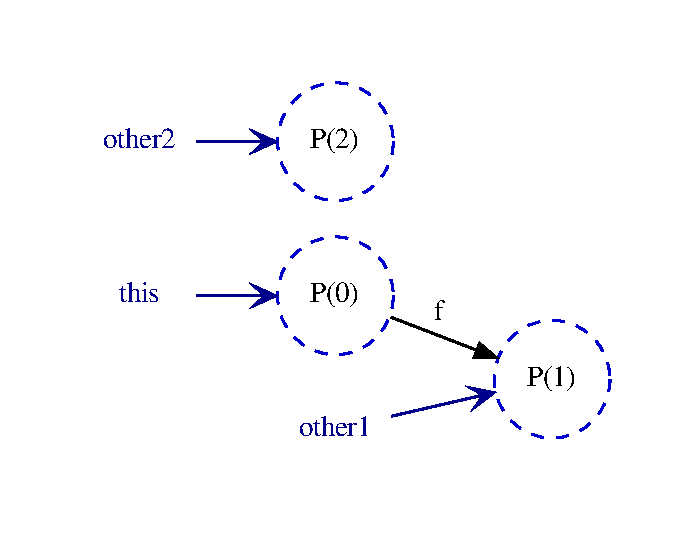
\includegraphics[scale=0.4]{images/pt_join1b1}} &
            \subfloat[Branch 2]{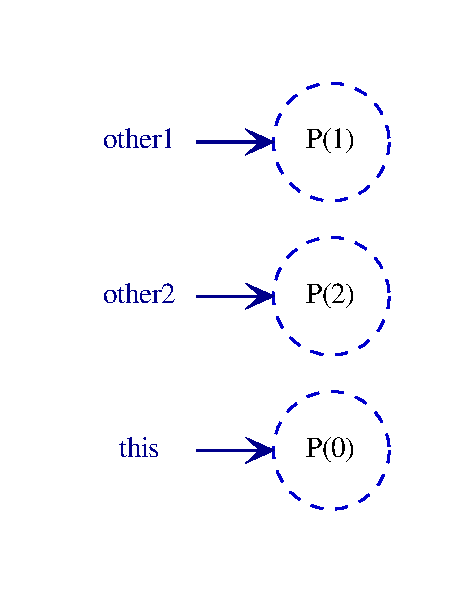
\includegraphics[scale=0.4]{images/pt_join1b2}}
        \end{tabular} \\
    \subfloat[Result]{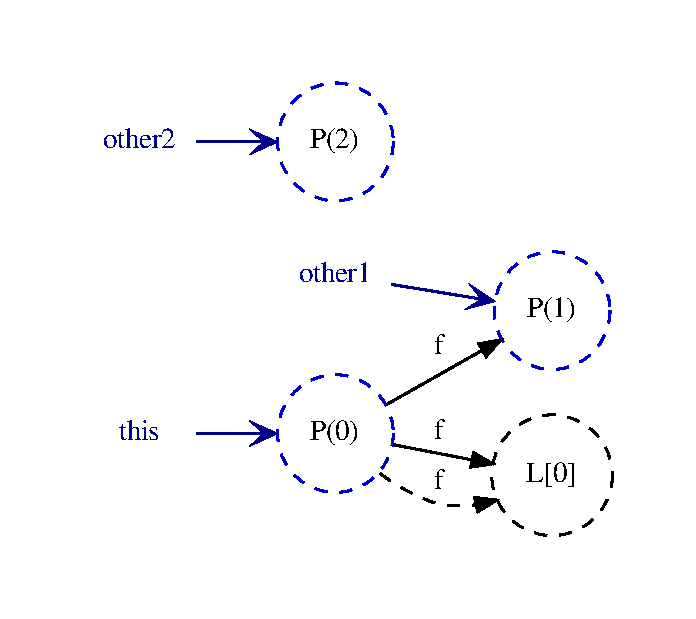
\includegraphics[scale=0.4]{images/pt_join1res}}
    \end{tabular}
\end{minipage}
    \caption{Example 1: introduction of a load node}
    \label{fig:pt:join1}
\end{figure}

\paragraph{Example 2}
Figure~\ref{fig:pt:join2} contains a conditional update, preceded by a
write on the same field. In this case, no load node needs to be introduced.
\begin{figure}[h]
\begin{minipage}[tl]{0.6\linewidth}
    \centering
\lstset{linewidth=0.6\linewidth}
\begin{lstlisting}
class A {
  var f: A = null
  def test(other1: A, other2: A) {
    this.f = other1
    if ( .. ) {
      this.f = other2 // Branch 1
    } else {
                     // Branch 2
    }
                     // Result
  }
}
\end{lstlisting}
\end{minipage}
\begin{minipage}[tr]{0.5\linewidth}
    \centering
    \begin{tabular}{c}
        \begin{tabular}{c c}
            \subfloat[Branch 1]{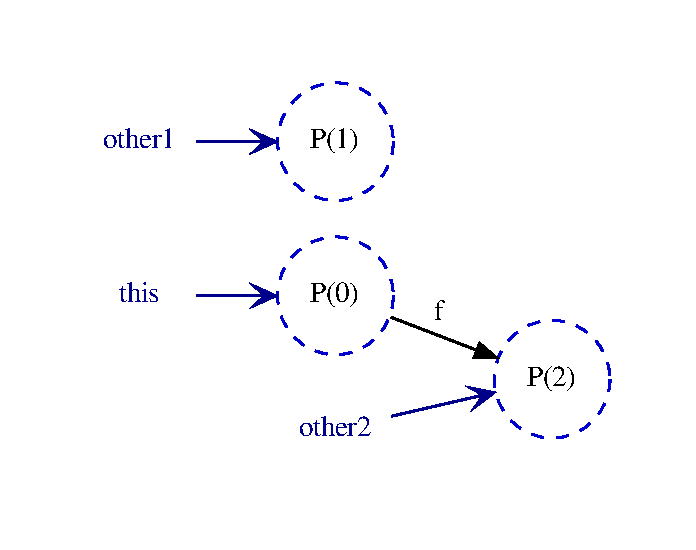
\includegraphics[scale=0.4]{images/pt_join2b1}} &
            \subfloat[Branch 2]{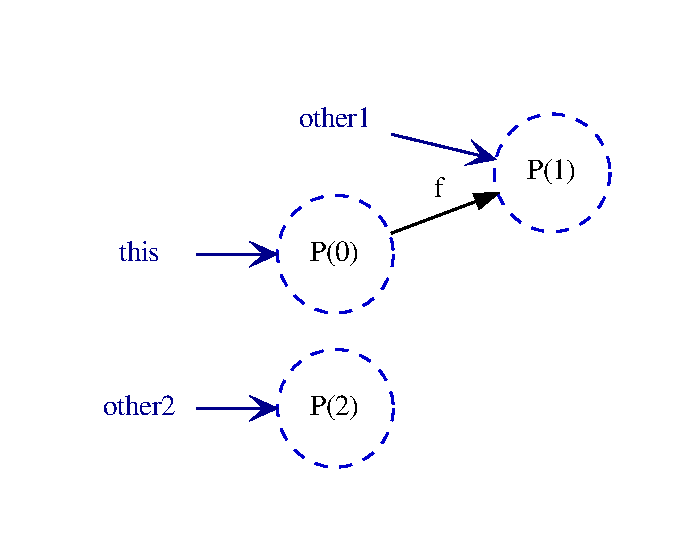
\includegraphics[scale=0.4]{images/pt_join2b2}}
        \end{tabular} \\
    \subfloat[Result]{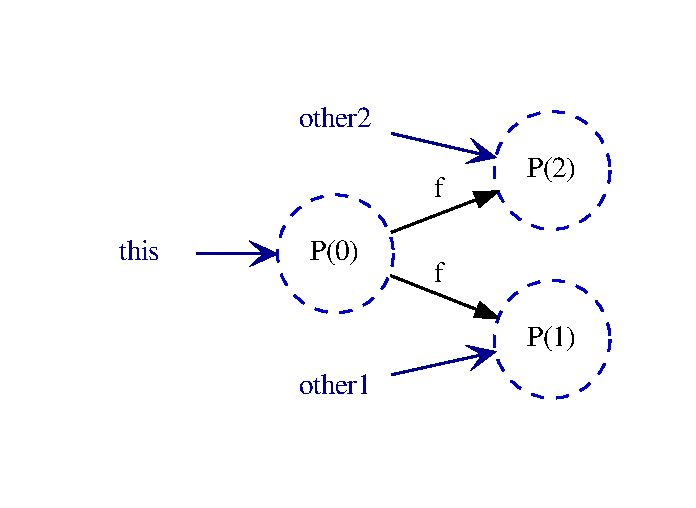
\includegraphics[scale=0.4]{images/pt_join2res}}
    \end{tabular}
\end{minipage}
    \caption{Example 2: Strong update followed by a conditional update}
    \label{fig:pt:join2}
\end{figure}

\paragraph{Example 3}
Figure~\ref{fig:pt:join3} illustrate the case of a conditional write on the
same field with the same \emph{source} node, but with distinct destinations. We
are able to establish that after this conditional update, $this.f$ no longer
retain its old value. This code is equivalent to the previous example, and
indeed yields the same effects.
\begin{figure}[h]
\begin{minipage}[tl]{0.6\linewidth}
    \centering
\lstset{linewidth=0.6\linewidth}
\begin{lstlisting}
class A {
  var f: A = null
  def test(other1: A, other2: A) {
    if ( .. ) {
      this.f = other1 // Branch 1
    } else {
      this.f = other2 // Branch 2
    }
                     // Result
  }
}
\end{lstlisting}
\end{minipage}
\begin{minipage}[tr]{0.5\linewidth}
    \centering
    \begin{tabular}{c}
        \begin{tabular}{c c}
            \subfloat[Branch 1]{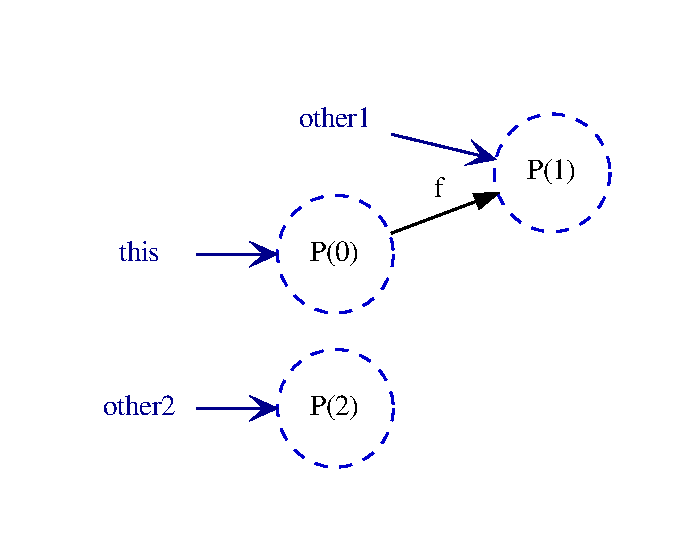
\includegraphics[scale=0.4]{images/pt_join3b1}} &
            \subfloat[Branch 2]{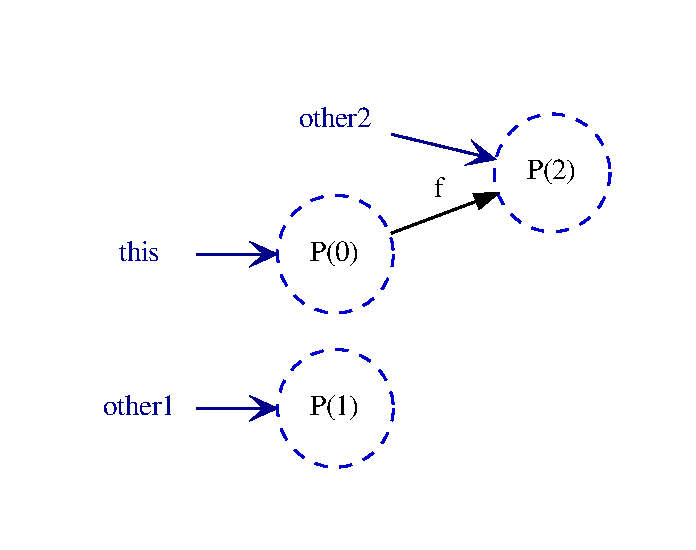
\includegraphics[scale=0.4]{images/pt_join3b2}}
        \end{tabular} \\
    \subfloat[Result]{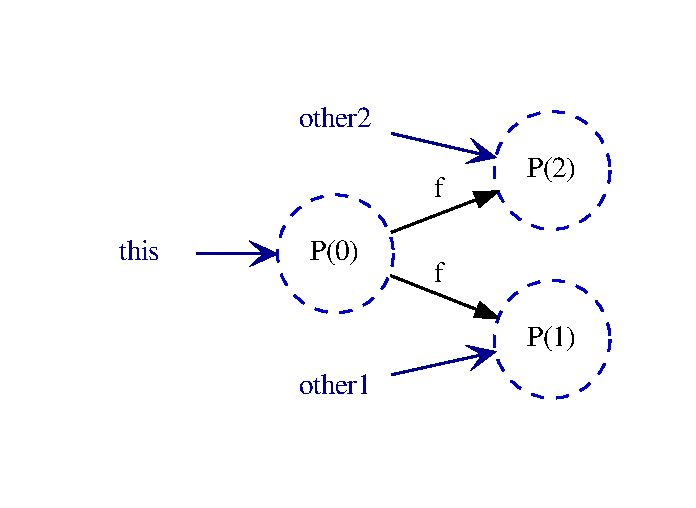
\includegraphics[scale=0.4]{images/pt_join3res}}
    \end{tabular}
\end{minipage}
    \caption{Example 3: two conditional strong updates}
    \label{fig:pt:join3}
\end{figure}
\FloatBarrier
\section{Graph-based Type Analysis}
Even though our global type analysis was flow sensitive, it suffered from
critical imprecision with respect to fields and arguments. For this reason, we
implemented a type analysis based on our graphs. The approach we took is to
attach type information to each node. Since nodes represent objects, this is a
sensible thing to do. The additional information we store alongside each node
is similar to what we used in our previous type analysis: $\langle T_{sub}, T_{ex} \rangle$
a pair of two sets of types $T_{sub}$ and $T_{ex}$ where $T_{sub}$ represents
the set of types from which we need to include subtypes, and $T_{ex}$.
The set of runtime types attached to each node is determined based on the node
types. Figure~\ref{fig:pt:types} illustrates the main cases. We then use those
types in order to compute the set of potential targets for a method call. Given
the call \verb/obj.foo()/, we obtain the set of runtime types corresponding to
\verb/obj/ as follows:
$$
    types(\verb/obj/) = \bigcup \{ \gamma(types(n)) ~|~ n \in nodes(\verb/obj/) \}
$$
we can then look for potential targets in the resulting set of types, similarly
to what we did in our previous type analysis.

\begin{figure}[h]
    \centering

    \begin{tabular}{ l | l }
        Node Type & Types Associated \\
        \hline
        INode(A)           & $\langle \emptyset, \{A\}\rangle$ \\
        LNode(a, f)        & $\langle\{type(a.f)\}, \{type(a.f)\}\rangle$ \\
        PNode(arg)         & $\langle\{type(arg)\}, \{type(arg)\}\rangle$ \\
        OBNode(A)          & $\langle \emptyset,   \{A\}\rangle$ \\
        NNode              & $\langle \emptyset,   \emptyset \rangle$ \\
        GBNode             & $\langle\{Object\},   \{Object\}\rangle$ (all)\\
        Literal Nodes      & $\langle \emptyset,   \{type(Literal)\}\rangle$\\
    \end{tabular}

    \caption{Summary: types associated to each kind of nodes}
    \label{fig:pt:types}
\end{figure}

If we pessimistically consider that each field read yield a \emph{load node},
and that every arguments become \emph{parameter nodes}, this type analysis is
exactly as precise as the one described previously. The main improvements comes
from two sides:
\begin{itemize}
    \item In practice, not every field reads yield a load node, for instance, a
read performed after a strong update will only return the newly assigned value,
which might be of a more precise set of types.
    \item When inlining those graphs, parameter nodes are mapped to other nodes
at the call site, and load nodes are resolved, if possible. The natural
inlining of methods makes this type analysis context sensitive. 
\end{itemize}
We consider in Figure~\ref{fig:pt:precise} an example illustrating this
improvement in precision.

\begin{figure}[h]
    \centering
\begin{lstlisting}
class A {
  var f: A = null
  def setF(a: A) { f = a }

  def test(obj: A) {
    val a = new A
    a.setF(a)
    a.f.foo()
  }
  def foo() {
    println("A")
  }
}

class B extends A {
  override def foo() {
    println("B")
  }
}
\end{lstlisting}
    \caption{Improved type analysis}
    \label{fig:pt:precise}
\end{figure}

At the time of the call to \verb/a.f.foo()/ we have from the graph at that
program point that \verb/a.f/ is the \emph{inside node} corresponding to the
object from \verb/new A/. We thus obtain $\langle \{\}, \{A\} \rangle$ for \verb/a.f/ instead of
$\langle \{A\}, \{A\} \rangle$, which excludes $B.foo$ from the call.
\section{Transfer Function}
We now describe  in Figure~\ref{fig:pt:tf} the transfer function illustrating
the transformations to the environment caused by most relevant statements. For
complex operations, we describe their effect in a specific function.

\begin{figure}[h]
    \centering

    \begin{tabular}{ l | l }
        Statement $st$                & Transfer Function $\emph{f}$\\
        \hline
        \verb/r = v/                     & $\langle N, E, locVar[r \mapsto nodes(v)], R \rangle$ \\
        \verb/r = new C/ @p              & $alloc(G, r, C, @p)$ \\
        \verb/r = null/                  & $\langle N \cup \{NNode\}, E, locVar[r \mapsto \{ NNode \}], R \rangle$ \\
        \verb/r.f = v/ @p                & $write(G, nodes(r), f, nodes(v), @p)$ \\
        \verb/r = v.f/ @p                & $read(G, nodes(v), f, r, @p)$ \\
        \verb/r = v.meth(a1, .., an)/ @p & $call(G, r, v, meth, (a_1, ..., a_n))$ \\
        \verb/return v/                  & $\langle N, E, locVar, nodes(v) \rangle$ \\
    \end{tabular}

    \caption{Transfer function $\emph{f}$}
    \label{fig:pt:tf}
\end{figure}

\subsection{Allocations}
The $alloc(Graph, r, C, @p)$ operation is responsible for creating the
appropriate inside node for the class $C$ and assign it to $r$. $@p$ represents
the program point at which the allocation occurs, in other words it represents
the allocation site.

During allocation, we also need to determine the \emph{singleton} flag of the
corresponding INode. There are two ways of generating inside nodes
corresponding to multiple objects: loops and function calls. We provide here
the general idea that will be able to handle both cases soundly. A refinement
of this technique in the presence of function calls will be described in
Section~\ref{sec:pt:allocinline}.

Algorithm~\ref{algo:pt:alloc} describe the transformations made to the graph by
$alloc$. The idea is simple: before actually including the corresponding inside
node into the environment, we look whether it is already present. In such case,
we are in the presence of a loop, and this inside node neds to get replaced by
a \emph{non-singleton} inside node. Otherwise, we add the inside node with
\emph{singleton} set to \emph{true}.

\begin{algorithm}
\caption{Allocations}\label{algo:pt:alloc}
\begin{algorithmic}[1]
\Function{alloc}{$\langle N, E, locVar, R \rangle, r, C, @p$}
    \State $n       \gets INode(C, false, @p)$
    \State $n_{sgt} \gets INode(C, true, @p)$

    \If{$n_{sgt} \in N$}
        \State $N_{new} \gets (N \cup \{ n \}) - \{ n_{sgt} \}$
        \State $locVar_{new} \gets \{ v \mapsto v_{nodes}[n_{sgt} \mapsto n] ~|~ (v \mapsto v_{nodes}) \in locVar \}$
        \State $locVar_{new} \gets locVar_{new}[ r \mapsto \{n\}]$
    \Else
        \State $N_{new} \gets N \cup \{ n_{sgt} \}$
        \State $locVar_{new} \gets locVar[ r \mapsto \{n_{sgt}\}]$
    \EndIf
    \State \Return $\langle N_{new}, E, locVar_{new}, R \rangle$
\EndFunction
\end{algorithmic}
\end{algorithm}

\subsection{Field Updates}
The $write(Graph, from, f, to, @p, allowStrong)$ operation is responsible for
managing field updates. It represents the modifications done by writing the nodes $to$ to
the field $f$ of nodes $from$, at program point $@p$. The $allowStrong$
argument specifies whether strong updates can be performed by this write
operation. The use for this argument will only become apparent for method
calls.

Algorithm~\ref{algo:pt:writes} describes the required graph transformations.
The main idea is that in case of a strong update, we simply remove old inside
edges and add the new one. It gets more complicated in the case of weak updates
since we need to keep the old value around. To determine the old value, we start
by following inside edges. If none exist, we follow outside edges. If this old
value is still not determined at this point, we introduce a load node to
represent it.

\begin{algorithm}
\caption{Field Updates}\label{algo:pt:writes}
\begin{algorithmic}[1]
\Function{write}{$\langle N, E, locVar, R \rangle, from, f, to, @p, allowStrong$}
    \State $isStrong \gets \forall n \in from.~ n.isSingleton \land |from| = 1 \land allowStrong$
    \State $N_{new} \gets N$

    \If{$isStrong$}
        \State $E_{new} \gets E - \{ ie ~|~ ie \in E \land ie \textsf{ is IEdge} \land ie.v1 \in from \land ie.f = f\} $
        \State $E_{new} \gets E_{new} \cup \{ IEdge(v_{from}, f, v_{to}) ~|~ v_{from} \in from \land v_{to} \in to \}$
    \Else
        \For{$n_{from} \gets from$}
            \State $previous \gets \{ ie.v2 ~|~ ie \in E \land ie \textsf{ is IEdge } \land ie.v1 = n_{from} \land ie.f = f \}$
            \State $E_{new} \gets E$
            \If{$previous = \emptyset$}
                \State $previous \gets \{ ie.v2 ~|~ oe \in E \land ie \textsf{ is OEdge } \land oe.v1 = n_{from} \land oe.f = f \}$
            \EndIf

            \If{$previous = \emptyset$}
                \State $lNode \gets safeLNode(n_{from}, f, @p)$
                \State $E_{new} \gets E_{new} \cup \{ IEdge(n_{from}, f, lNode), OEdge(n_{from}, f, lNode) \}$
                \State $N_{new} \gets N_{new} \cup \{ lNode \}$
            \EndIf


            \State $E_{new} \gets E_{new} \cup \{ IEdge(n_{from}, f, v_{to}) ~|~  v_{to} \in (previous \cup to) \}$
        \EndFor
    \EndIf
    \State \Return $\langle N_{new}, E_{new}, locVar, R \rangle$
\EndFunction
\end{algorithmic}
\end{algorithm}
\subsection{Field Reads}
The $read(Graph, to, f, from, @p)$ operation is responsible for
managing field reads. It represents the modifications done by reading the field
$f$ from the nodes $from$ and assigning the result to $to$, at program point
$@p$.

Algorithm~\ref{algo:pt:reads} describes the transformations done by $read$.
Intuitively, $read$ will try to determine a previous value by first following
$write$ and then $read$ edges. If no such value can be found, it will introduce
a load node representing this value.

\begin{algorithm}
\caption{Field Reads}\label{algo:pt:reads}
\begin{algorithmic}[1]
\Function{read}{$\langle N, E, locVar, R \rangle, from, f, to, @p$}
    \State $N_{new} \gets N$
    \State $E_{new} \gets E$
    \State $pointed \gets \emptyset$

    \For{$n_{from} \gets from$}
        \State $previous \gets \{ ie.v2 ~|~ ie \in E \land ie \textsf{ is IEdge } \land ie.v1 = n_{from} \land ie.f = f \}$
        \If{$previous = \emptyset$}
            \State $previous \gets \{ ie.v2 ~|~ oe \in E \land ie \textsf{ is OEdge } \land oe.v1 = n_{from} \land oe.f = f \}$
        \EndIf

        \If{$previous = \emptyset$}
            \State $lNode \gets safeLNode(n_{from}, f, @p)$
            \State $E_{new} \gets E_{new} \cup \{ OEdge(n_{from}, f, lNode) \}$
            \State $N_{new} \gets N_{new} \cup \{ lNode \}$
            \State $pointed \gets pointed \cup \{ lNode \}$
        \Else
            \State $pointed \gets pointed \cup previous$
        \EndIf
    \EndFor

    \State \Return $\langle N_{new}, E_{new}, locVar[ to \mapsto pointed, R \rangle$
\EndFunction
\end{algorithmic}
\end{algorithm}
\subsection{Load Nodes Creation}
In the previous algorithms, we used a $safeLNode$ function that is responsible
to \emph{safely} create new load nodes so that it still allows the analysis
to terminate. For example, if $safeLNode(from, field, @p)$ was naively creating
a new $LNode(from, field, @p)$, the analysis would not necessarily terminate!

\begin{figure}[h]
\begin{lstlisting}
class A (next: A) {
  def traverse = {
    val current = this
    while(current != null) {
      current = current.next // @p
    }
  }
}
\end{lstlisting}
    \caption{Problematic code with respect to load nodes}
    \label{fig:pt:lnodeloop}
\end{figure}

We now walk through our analysis to illustrate why it would not terminate with
such a definition of $safeLNode$, given the code provided in
Figure~\ref{fig:pt:lnodeloop}:
\begin{enumerate}
    \item After the first iteration, the read will have created the load node \\
    $l_1 := LNode(P(0), next, @p)$, since $P(0).next$ was yet undetermined.
    \item At the beginning of the second iteration, we have $nodes(current) =
    \{ P(0), l_1 \}$.
    \item After the second iteration, the read will have created the load node
    $l_2 := LNode(l_1, next, @p)$, since $l_1.next$ or  $P(0).next.next$ was
    undetermined.
    \item And so on, a new load node is created at each iteration, the analysis
    is thus unable to terminate.
\end{enumerate}

In order to solve this issue, we need to limit the way we generate new load
nodes, so that their number is always bounded.
Algorithm~\ref{algo:pt:safelnode} describes how we defined $safeLNode$ in such
a way.

\begin{algorithm}
\caption{Safely Creating Load Nodes}\label{algo:pt:safelnode}
\begin{algorithmic}[1]
\Function{safeLNode}{$from, f, @p$}
    \If{$from \textsf{ is LNode}$}
        \State $from_{new} \gets from.from$
    \Else
        \State $from_{new} \gets from$
    \EndIf

    \State \Return $LNode(from_{new}, f, @p)$
\EndFunction
\end{algorithmic}
\end{algorithm}

\subsection{Method Calls}
\label{sec:pt:inlining}
For method calls, the effects of the method are represented by the graph
resulting from the analysis of the function. The callgraph computed after
type analysis allows us to group inter-dependent functions together (in
strongly connected components). We can then perform a topological sort of
those strongly connected components, which will basically order the analysis
in such a way that most methods will already have been analyzed when
encountering one of their call sites.

We describe in Algorithm~\ref{algo:pt:meth1} how we handle statements
representing method calls. Given the statement $r = v.meth(a_1, .., a_n)$,
we first need to resolve the types corresponding to $v$, so that we can
collect all methods $meth$ that might be the targets of this call. We then
\emph{inline} the graph for each target separately, and then join the resulting
environments.

\begin{algorithm}
\caption{Method Call}\label{algo:pt:meth1}
\begin{algorithmic}[1]
\Function{call}{$G, r, v, meth, (arg_1, ..., arg_n), @p$}
    \State $types_{rec} \gets resolve(types(v))$
    \State $methods \gets \{ m ~|~ T \in types_{rec} \land m \in methods(T) \land m.name = meth.name \}$
    \State $nodes_{rec} \gets nodes(v)$
    \State $nodes_{args} \gets (r_1, ..., r_n) ~~\textsf{ s.t.}~~ r_i = nodes(arg_i)$
    \State \Return $\bigsqcup ~\{~ inlineGraph(G, m, Graphs(m), nodes_{rec}, nodes_{args}, @p) ~|~ m \in methods \}$
\EndFunction
\end{algorithmic}
\end{algorithm}

\begin{algorithm}
\caption{Graph Inlining}\label{algo:pt:meth1}
\begin{algorithmic}[1]
\Function{inlineGraph}{$G_{caller}, meth, G_{callee}, recNodes, argsNodes, @p$}
    \State $\langle map, G_{new} \rangle \gets buildMap(G_{caller}, meth, G_{callee}, recNodes, argsNodes, @p)$
    \Repeat
        \State $G_{old} \gets G_{new}$

        \State $mapEdges \gets \{ \langle IEdge(mv_1, e.f, mv_2), e.v_1 \rangle
        ~|~ e \in G_{callee}.E \land e \textsf{ is IEdge} \land mv_1 \in
        map(e.v_1) \land mv_2 \in map(e.v_2) \}$

        \State $sources \gets \{ \langle e.v_1, e.f \rangle ~|~ \langle e, o \rangle \in mapEdges \}$

        \For {$\langle v, f \rangle \gets sources$}
            \State $edges \gets \{ e ~|~ \langle e, o \rangle \in mapEdges \land \langle e.v_1, e.f \rangle = \langle v, f\rangle \}$
            \State $olds  \gets \{ o ~|~ \langle e, o \rangle \in mapEdges \land \langle e.v_1, e.f \rangle = \langle v, f\rangle \}$

            \State $allowStrong \gets \forall o \in olds~.~|map(o)| = 1$

            \State $G_{new} \gets write(G_{new}, \{ v \}, f, \{ e.v_2 ~|~ e \in edges \}, @p, allowStrong)$
        \EndFor
    \Until{$G_{new} = G_{old}$}
\EndFunction
\end{algorithmic}
\end{algorithm}

The formal description of the inlining algorithm is rather complex, but its
intuition is relatively easy to understand: we start by mapping each write
operations from the callee to corresponding write operations in the caller,
using the previously computed $map$. Once we have the corresponding write
operations grouped by the node and field they affect, it remains to determine
whether this write operation could be strong. Given a write on $v.f$, a
strong update is allowed if $v$ was only pointed to from the callee by nodes
with $v_1$ as unique target in the map. In other words, if 
$$
\forall v_{orig} \in map^{-1}(v)~.~ map(v_{orig}) = \{ v \}
$$
It is worth noting that allowing a strong update at this stage does not
necessarily mean that a strong update will indeed be performed. It is only
enabling the $write$ operation to perform one if it sees fit to do so.

\subsubsection{Mapping Nodes Between Graphs}
\label{sec:pt:allocinline}
For this inlining to be fully defined, it remains to describe how this $map$ is
initially computed. Algorithm~\ref{algo:pt:map} describes how this mapping is
performed. It trivially starts by mapping nodes corresponding to the parameters
of the function, including the 0th argument representing the receiver. All
global nodes are also mapped to themselves.

For \emph{inside nodes}, we first precise the allocation site by composing it
with the point at which the method is called, we do it in a way such that no
repetitions are allowed. Otherwise, it would not terminate in the case of a
recursive function. We also, like in the case of an allocation statement,
figure out this node's \emph{singleton} flag, by detecting loops. In case we
previously had a \emph{singleton} node and detected a cycle, we replace it with
a \emph{non-singleton} node and adjust the map accordingly.
\begin{algorithm}
\caption{Building Node Map}\label{algo:pt:map}
\begin{algorithmic}[1]
\Function{buildMap}{$G_{caller}, meth, G_{callee}, recNodes, argsNodes, @p$}
    \State $G_{new} \gets G_{caller}$
    \State $map \gets \{ P(0) \mapsto recNodes \} $
    \For {$i \gets 1 ~to~ |meth.args|$}
        \State $map = map \cup \{ P(i) \mapsto argsNodes_i \}$
    \EndFor
    \For {$n \in LitNodes \cup OBNodes \cup \{NNode, GBNode\}$}
        \State $map = map \cup \{ n \mapsto \{ n \} \}$
    \EndFor
    \For {$in \in \{ n ~|~ n \in G_{callee}.N \land n \textsf{ is INode}\}$}
        \State $pPoint \gets compose(n.pPoint, @p)$
        \State $iNode_{sgt} \gets INode(types(in), true, pPoint)$
        \State $iNode \gets INode(types(in), false, pPoint)$

        \If {$iNode_{sgt} \in G_{new}.N \lor iNode \in G_{new}.N$}
            \State $G_{new}.N \gets (G_{new}.N \cup \{ iNode \}) - \{ INode_{sgt} \}$
            \State $map \gets map[iNode_{sgt} \mapsto iNode] \cup \{in \mapsto \{iNode\}\}$
        \Else
            \State $G_{new}.N \gets G_{new}.N \cup \{ iNode_{sgt} \}$
            \State $map \gets map \cup \{in \mapsto \{iNode_{sgt}\}\}$
        \EndIf
    \EndFor
    \For {$ln \in \{ n ~|~ n \in G_{callee}.N \land n \textsf{ is LNode}\}$}
        \State $\langle map, G_{new} \rangle = resolveLoad(ln, map, G_{new}, @p)$
    \EndFor
    \State \Return $\langle map, G_{new} \rangle$
\EndFunction
\end{algorithmic}
\end{algorithm}

In the presence of \emph{load nodes}, we need to see if they are fully
determined in the caller graph, so that we can resolve them. The resolution will
be made from their \emph{from} node. Since this node could itself be a yet
unresolved load node, we first make sure that it is resolved by calling
$resolveLoad$ on it. As in the case of a read operation, we follow first inside
and then outside edges. If no target is found, we need to maintain the node in
the resulting graph. Here again, we safely refine its program point.

\begin{algorithm}
\caption{Resolving Load Nodes}\label{algo:pt:resload}
\begin{algorithmic}[1]
\Function{resolveLoad}{$lNode, map, G, @p$}

    \State $LNode(from, f, pPoint) \gets lNode$

    \If {$from \textsf{ is LNode}$}
        \State $\langle map, G \rangle = resolveLoad(from, map, G, @p)$
    \EndIf

    \For {$n \in map(from)$}
        \State $targets \gets \{ ie.v2 ~|~ ie \in G.E \land ie \textsf{ is IEdge } \land ie.v1 = n \land ie.f = f \}$
        \If{$targets= \emptyset$}
            \State $targets \gets \{ ie.v2 ~|~ oe \in G.E \land ie \textsf{ is OEdge } \land oe.v1 = n \land oe.f = f \}$
        \EndIf

        \If{$targets= \emptyset$}
            \State $pPoint \gets compose(pPoint, @p)$
            \State $newLNode \gets safeLNode(from, f, pPoint)$
            \State $G.E \gets G.E \cup \{ IEdge(n, f, newLNode), OEdge(n, f, newLNode) \}$
            \State $G.N \gets G.N \cup \{ newLNode \}$
            \State $map \gets map \cup \{ lNode \mapsto \{ newLNode \} \}$
        \Else
            \State $map \gets map \cup \{ lNode \mapsto targets \}$
        \EndIf
    \EndFor

    \State \Return $\langle map, G \rangle$
\EndFunction
\end{algorithmic}
\end{algorithm}

\subsection{Analysis Inter-dependant and Recursive Methods}
As explained earlier, we analyze groups of inter-dependent functions together.
They are represented by non-singleton strongly-connected components in our
call-graph.  We construct the effects of the methods iteratively, assuming that
methods have initially no effect (i.e. their effect graph is empty). The
algorithm for the analysis of SCCs is outlined in
Algorithm~\ref{algo:pt:interdep} and consists of a standard fix-point
mechanism.

\begin{algorithm}
\caption{Resolving Load Nodes}\label{algo:pt:interdep}
\begin{algorithmic}[1]
\Function{analyzeSCC}{$scc:\{m_1, ..., m_n \}$}
    \State $workList \gets scc$

    \While {$|workList| > 0$}
        \State $m ~s.t.~ m \in workList$
        \State $workList \gets workList - m$

        \State $G_{before} \gets Graphs(m)$
        \State $analyze(m)$
        \State $G_{after} \gets Graphs(m)$

        \If {$G_{before} \neq G_{after}$}
            \State $workList \gets workList \cup \{ t ~|~ \textsf{ t calls m } \}$
        \EndIf
    \EndWhile

\EndFunction
\end{algorithmic}
\end{algorithm}

\section{Argument for Termination}
\section{Loop/Function Equivalence}
Even though Scala can be used pretty much like an imperative language, its
features favor functional programming. It is thus critical to provide
a precise inter-procedural analysis. We demonstrate in this section that
loops and their corresponding functional version are equivalently represented
as graphs. For instance, Figure~\ref{fig:equiv:code} provides two equivalent
implementations of the same code, one imperative and one functional.

\begin{figure}[h]
\begin{minipage}[t]{0.5\linewidth}
    \centering
\begin{lstlisting}
val c: Constants = initConstants
var s: State = initState
while(cond(s, c)) {
    s = update(s, c)
}
s
\end{lstlisting}
\end{minipage}
\begin{minipage}[t]{0.5\linewidth}
    \centering
\begin{lstlisting}
def f(s : State, c : Constants) : State = {
 if(cond(s, c)) {
   f(update(s, c), c)
 } else {
   s
 }
}
f(initState, initConstants)
\end{lstlisting}
\end{minipage}
    \caption{Two equivalent implementations, for arbitrary functions $cond$ and $update$}
    \label{fig:equiv:code}
\end{figure}

We expect from the effect graphs to be the same. Indeed, it would be profitable
for two main reasons:
\begin{itemize}
    \item Scala will translate certain call patterns into while loop for
efficiency reasons. And thus, the inference of the effects of a while loop
should be well handled.

    \item Since Scala encourages functional programming, a tool targeted at
Scala programs is expected to be precise in presence of functional code, and
notably recursive function calls.
\end{itemize}

We argue informally by comparing the fix-point technique used in a loop and the
fix-point performed within a strongly connected component in the call-graph
(mutually recursive functions). First, let us introduce some recursive
$fixpoint$ function defined as:
\begin{eqnarray*}
    fixpoint(init, \mathcal{F})(0) &:=& init \\
    fixpoint(init, \mathcal{F})(n) &:=& fixpoint(init, \mathcal{F})(n-1) \cup \mathcal{F}(fixpoint(init, \mathcal{F})(n-1)) \\
\end{eqnarray*}

\paragraph{Loop Fix-Point}
We start by assuming that the effects of the entire looping block (in this case
the effects of \verb/s = update(s, c)/) are compacted into one specific
transfer function $\mathcal{F}$, mapping the state at the entry of the loop to
the state at the end. Given a state $S$ before the loop, we obtain $S$ after 0
iterations, and $S \cup \mathcal{F}(S)$ after one iteration. After two
iterations, we obtain $S \cup \mathcal{F}(S) \cup \mathcal{F}(S \cup
\mathcal{F}(S))$ which corresponds to $fixpoint(S, \mathcal{F})(2)$. Naturally,
after $n$ iterations we get $fixpoint(S, \mathcal{F})(n)$.

\paragraph{Function Fix-Point}
When handling mutually recursive functions, we start by assuming functions have
no effect. We then analyze each function until the graph of every functions in
the strongly connected component are stable. In the present case, we start by
analyzing $f$ assuming that $f$ has yet no effect. The first call to $f$
produces thus no effect.

At the end of this first analysis, we obtain the initial state $S$ which is
given by the first parameter. The second analysis will thus consider a function
returning its first argument as effect, and thus the effect of the call will be
again $\mathcal{F}(S)$. Joined with the other effect-less branch, we obtain $S
\cup \mathcal{F}(S)$. A subsequent iteration will yield: $S \cup \mathcal{F}(S)
\cup \mathcal{F}(S \cup \mathcal{F}(S)) = fixpoint(S, \mathcal{F})(2)$. After
$n$ recursive call, we again obtain $fixpoint(S, \mathcal{F})(n)$.

\paragraph{}
Provided that $\mathcal{F}$ is monotonic (which is the case given that it is
a composition of calls to our transfer function), and that our lattice does not
allow infinite ascending chains, we have that $fixpoint(S, \mathcal{F})(\infty)$
exists.

We have thus informally established that both kinds of fix-point will yield the
same effects. And thus, both flavors of programming will yield equivalent
results.

